% Standalone TikZ figure for ZenBrain architecture
% Compile separately: pdflatex architecture.tex
% Then include as: \includegraphics[width=\textwidth]{figures/architecture.pdf}
\documentclass[tikz,border=5pt]{standalone}
\usepackage[T1]{fontenc}
\usetikzlibrary{arrows.meta, positioning, calc, fit, backgrounds}

\definecolor{working}{RGB}{254, 215, 102}    % warm yellow
\definecolor{shortterm}{RGB}{253, 186, 116}  % orange
\definecolor{episodic}{RGB}{147, 197, 253}   % light blue
\definecolor{semantic}{RGB}{134, 239, 172}   % green
\definecolor{procedural}{RGB}{196, 181, 253} % purple
\definecolor{core}{RGB}{252, 165, 165}       % red/pink
\definecolor{crossctx}{RGB}{156, 163, 175}   % gray
\definecolor{coordinator}{RGB}{99, 102, 241} % indigo

\begin{document}
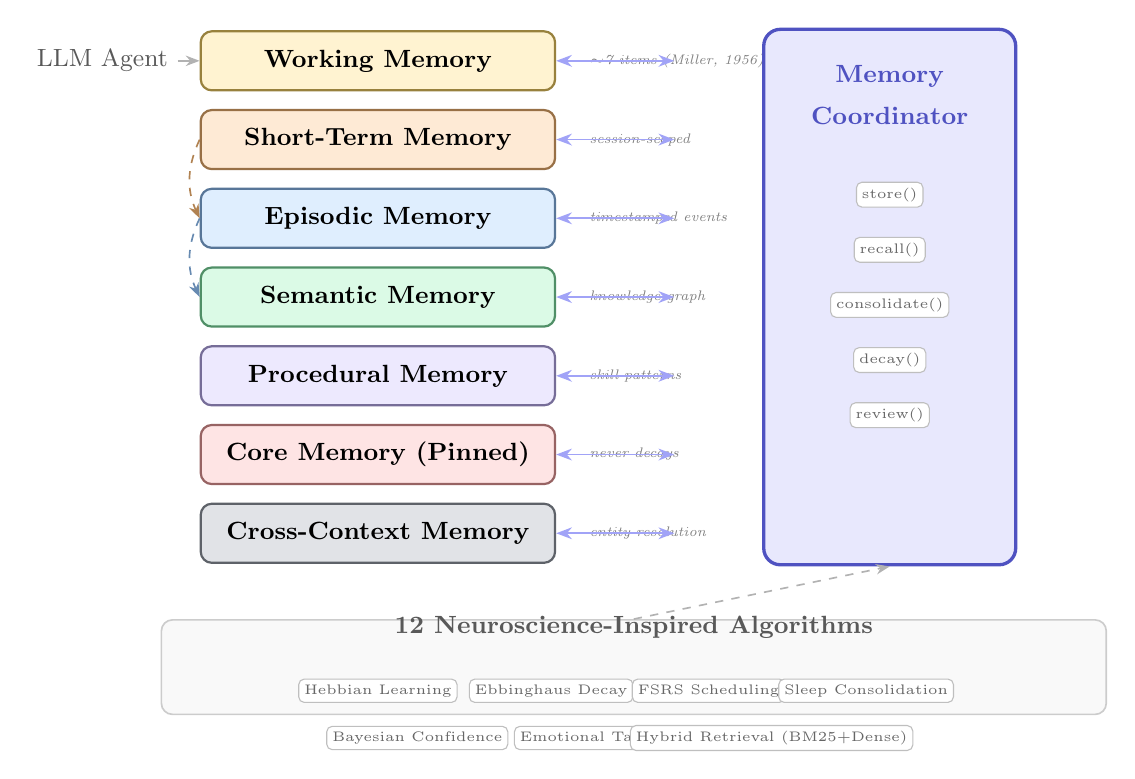
\begin{tikzpicture}[
    layer/.style={
        rectangle, rounded corners=4pt, draw=#1!60!black, fill=#1!30,
        minimum width=4.5cm, minimum height=0.75cm,
        font=\small\bfseries, text=black, line width=0.8pt
    },
    algo/.style={
        rectangle, rounded corners=2pt, draw=gray!50, fill=white,
        font=\tiny, text=gray!80!black, inner sep=2pt
    },
    op/.style={
        -{Stealth[length=5pt]}, line width=0.6pt, #1
    },
    >=Stealth
]

% Memory Layers (stacked)
\node[layer=working]    (wm)  at (0, 5.5) {Working Memory};
\node[layer=shortterm]  (stm) at (0, 4.5) {Short-Term Memory};
\node[layer=episodic]   (em)  at (0, 3.5) {Episodic Memory};
\node[layer=semantic]   (sm)  at (0, 2.5) {Semantic Memory};
\node[layer=procedural] (pm)  at (0, 1.5) {Procedural Memory};
\node[layer=core]       (cm)  at (0, 0.5) {Core Memory (Pinned)};
\node[layer=crossctx]   (xm)  at (0,-0.5) {Cross-Context Memory};

% Layer annotations (right side)
\node[right=0.3cm of wm, font=\tiny\itshape, text=gray] {$\sim$7 items (Miller, 1956)};
\node[right=0.3cm of stm, font=\tiny\itshape, text=gray] {session-scoped};
\node[right=0.3cm of em, font=\tiny\itshape, text=gray] {timestamped events};
\node[right=0.3cm of sm, font=\tiny\itshape, text=gray] {knowledge graph};
\node[right=0.3cm of pm, font=\tiny\itshape, text=gray] {skill patterns};
\node[right=0.3cm of cm, font=\tiny\itshape, text=gray] {never decays};
\node[right=0.3cm of xm, font=\tiny\itshape, text=gray] {entity resolution};

% MemoryCoordinator (right)
\node[rectangle, rounded corners=6pt, draw=coordinator!80!black, fill=coordinator!15,
      minimum width=3.2cm, minimum height=6.8cm, line width=1.2pt,
      font=\small\bfseries, text=coordinator!80!black]
      (coord) at (6.5, 2.5) {};
\node[font=\small\bfseries, text=coordinator!80!black] at (6.5, 5.3) {Memory};
\node[font=\small\bfseries, text=coordinator!80!black] at (6.5, 4.8) {Coordinator};

% Coordinator operations
\node[algo] (store)   at (6.5, 3.8) {store()};
\node[algo] (recall)  at (6.5, 3.1) {recall()};
\node[algo] (consol)  at (6.5, 2.4) {consolidate()};
\node[algo] (decay)   at (6.5, 1.7) {decay()};
\node[algo] (review)  at (6.5, 1.0) {review()};

% Algorithms (bottom)
\node[rectangle, rounded corners=4pt, draw=gray!40, fill=gray!5,
      minimum width=12cm, minimum height=1.2cm, line width=0.6pt]
      (algos) at (3.25, -2.2) {};
\node[font=\small\bfseries, text=gray!70!black] at (3.25, -1.7) {12 Neuroscience-Inspired Algorithms};

\node[algo] at (0, -2.5) {Hebbian Learning};
\node[algo] at (2.2, -2.5) {Ebbinghaus Decay};
\node[algo] at (4.2, -2.5) {FSRS Scheduling};
\node[algo] at (6.2, -2.5) {Sleep Consolidation};

\node[algo] at (0.5, -3.1) {Bayesian Confidence};
\node[algo] at (2.8, -3.1) {Emotional Tagging};
\node[algo] at (5.0, -3.1) {Hybrid Retrieval (BM25+Dense)};

% Arrows: Layers <-> Coordinator
\foreach \layer in {wm, stm, em, sm, pm, cm, xm} {
    \draw[op=coordinator!60, <->] (\layer.east) -- ++(1.5, 0);
}

% Arrows: Algorithms -> Coordinator
\draw[op=gray!60, dashed] (algos.north) -- (coord.south);

% Consolidation arrows between layers
\draw[op=shortterm!70!black, dashed, bend right=25]
    (stm.west) to node[left, font=\tiny, text=gray] {} (em.west);
\draw[op=episodic!70!black, dashed, bend right=25]
    (em.west) to node[left, font=\tiny, text=gray] {} (sm.west);

% Input/Output
\node[font=\small, text=gray!70!black] (input) at (-3.5, 5.5) {LLM Agent};
\draw[op=gray!60, thick] (input) -- (wm.west);

\end{tikzpicture}
\end{document}
